\chapter[Air-conditioning Systems]{Air-conditioning Systems}

Thermodynamics has gained a lot of attention since the Industrial Revolution, since this field contributes with the creation and improvement of different thermal machines - notably steam engines - and it still have a lot of relevance in the modern world. Every piece of technology around us has had contribution from thermodynamics for its creation. For this reason, even as society thinks that the Climate Change is a consequence of those technologies, we don't want to stop using it. 

There is a natural transfer of energy between warmer to colder bodies - this phenomena is known as heat. The heat transfer can occur by three different manners: radiation, convection and conduction. If two or more bodies don't exchange more heat, we consider that they are in thermal equilibrium. The heat exchange between substances can affect properties besides the temperature, as pressure or volume. Thermodynamics studies these sort of interactions \cite{Maxwell}.

Heat flows between bodies with higher temperature to the ones with lower - this is known as The Second Law of Thermodynamics. For this reason, machines like air-conditioning and refrigerators that tries to make heat flow in the opposite direction has a cost. These machines sometimes are called: inverse cycle thermal machines. They were theorize first by Sadi Carnot in the attempt to calculate the maximum efficiency of thermal machines. However, they ended up being actually used without the due attention with the rise of atmospheric entropy \cite{Carnot}. 

Sadi Carnot compared thermal machines to a waterfall - the top of the waterfall is the Heat Source and the bottom is the Cooling Source. This analogy helps with understanding the absurdity of trying to make heat flows its opposite way. It is possible with small amounts of energy, however if you analyze the whole system, heat will always flow its natural course the same way that the water of the waterfall will fall. On reality, there is not a great thermal insulation between the Heat and Cooling sources, which makes air-conditioning systems spend a lot of energy (\autoref{carnot}).

\begin{figure}[ht]
    \centering
    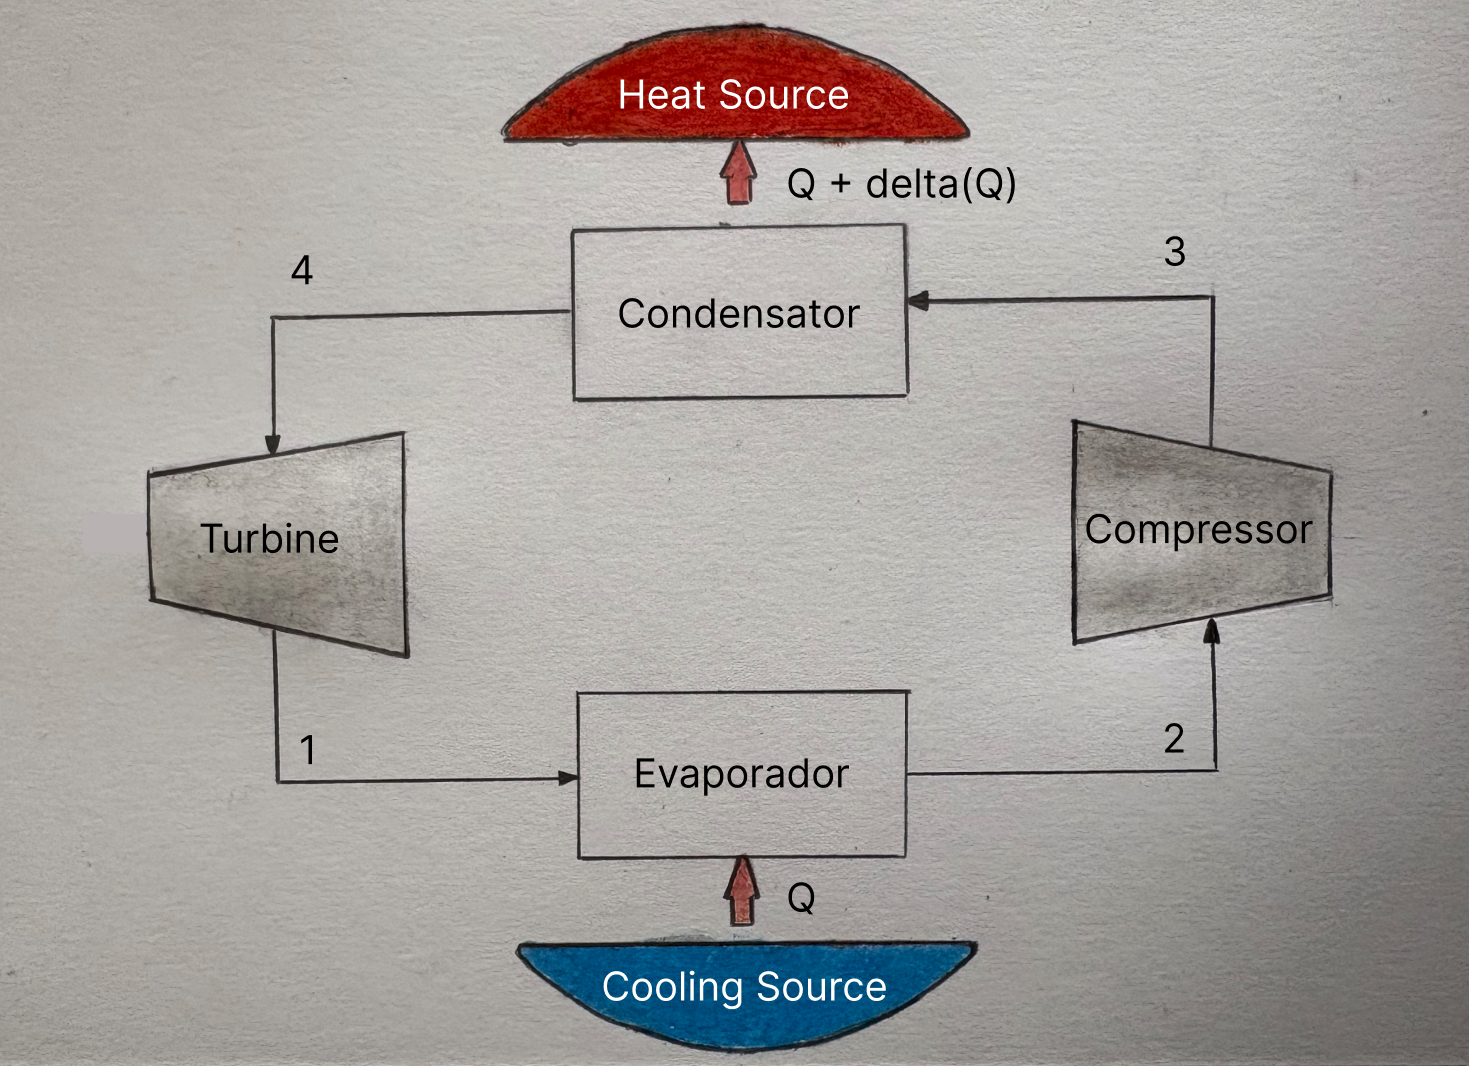
\includegraphics[scale=0.25]{pictures/carnot.png}
    \caption{Carnot's inverse cycle thermal machine  - would be an ideal refrigerator, but it is impossible on practise.}
    \label{carnot}
\end{figure}

On other words, air conditioning greatly influences the entropy of the atmosphere. Entropy was defined by Rudolf Clausius as the infinitesimal change in heat divided by instantaneous temperature. Sometimes it is known as the measurament of chaos in a system, so if the aim is climate stabilization, it's essential to be aware of machines that greatly increases this property \cite{Clausius}.

The air-conditioning system simply throws heat from a room to the outside, and in this process, some of the electric energy is converted in more thermal energy. Since heat flows its natural course, some of this thermal energy promptly returns to the room. Besides, since warmer air tends to rise due to its lower density, air-conditioning negatively affects upper floors in buildings. The lower floor neighbors' air-conditioning throws its heat to the outside, which tends to go upwards to the upper neighbors' flat. We are waisting energy using air-conditioning systems as refrigerator method (\autoref{predios}).

\begin{figure}[ht]
    \centering
    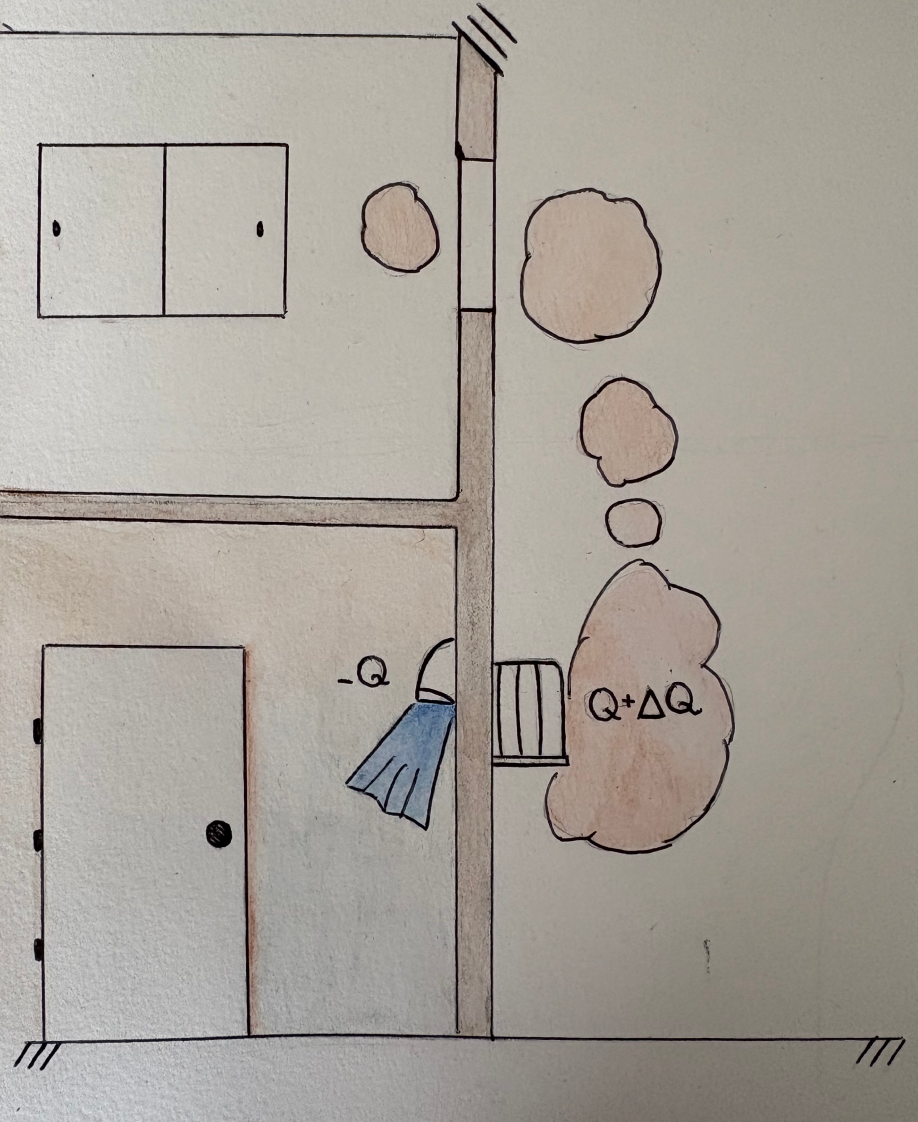
\includegraphics[scale=0.35]{pictures/predio.png}
    \caption{Air-conditioning system functioning - Increase of heat that flows back into the room and neighbors' homes.}
    \label{predios}
\end{figure}

A second analogy to air-conditioning systems is: removing water from a broken ship with a bucket. It does not solve the problem and it wastes a lot of energy. Air-conditioning systems are refrigerators with open doors: they might soothe the problem for the person in front of it, but for the overall system, it's efficiency is negative. \textbf{Besides, Global Warming is a public problem and its solution must also be in the public infrastructure. }
                                                                           
Carnot's thesis "Reflections on the Motive Power of Fire" considered the thermal machines as insulated from the environment, which is a comprehensive mistake since at the time there were no inverse cycle thermal machines in use. However, if we analyze the current urban systems with millions of these machines, we start to better understand the Climate Crisis.

When we analyze the system on a global scale, the air-conditioning use creates more thermal energy and increases the local atmospheric entropy. This generates a high pressure zone that is sometimes called Urban Heat Island (\autoref{ilha-calor}). Air-conditioning is not a room refrigerator, it is a \textbf{world heater}. The higher pressure on the urban heat islands expels clouds and decreases the likelihood of raining, since warmer temperatures requires more water for precipitation. In this manner, when it rains the amount of water is higher, increasing the risk of rainstorms, floods and hurricanes.

\begin{figure}[ht]
    \centering
    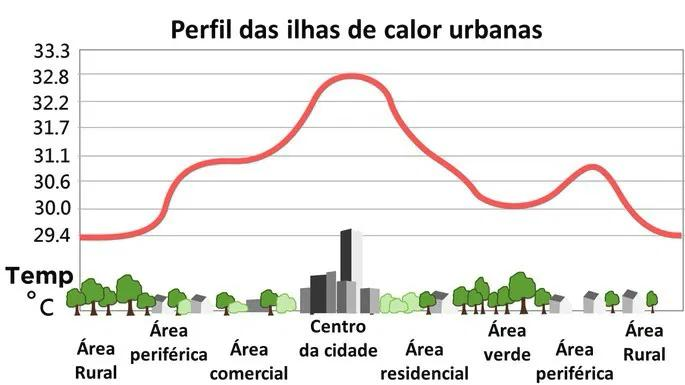
\includegraphics[scale=0.6]{pictures/ilha-calor.jpg}
    \caption{Ilustração da ilha de calor gerada pela alta queima de conbustível fóssil e refrigeração ineficiente.}
    \label{ilha-calor}
    \legend{Fonte: https://www.todamateria.com.br/ilha-de-calor/}
\end{figure}

It is an error to consider the atmosphere as a thermal reservoir as it is taught in engineering courses. It is true that it has a lot od thermal capacity when compared to daily life objects. However, society has hundreds of millions of air-conditioning systems working, which have the capacity to affect world's atmosphere. Besides, most of them are concentrated in urban areas. 
As a last argument, The air-conditioning systems loses efficiency when it is too warm, so when people most need a refrigerator system, it will consume more energy. 